%!TEX root = nextndnvideo-tr.tex
\section{prior work} % (fold)
\label{sec:comparison}
\begin{figure}%[htbp]
  \centering
  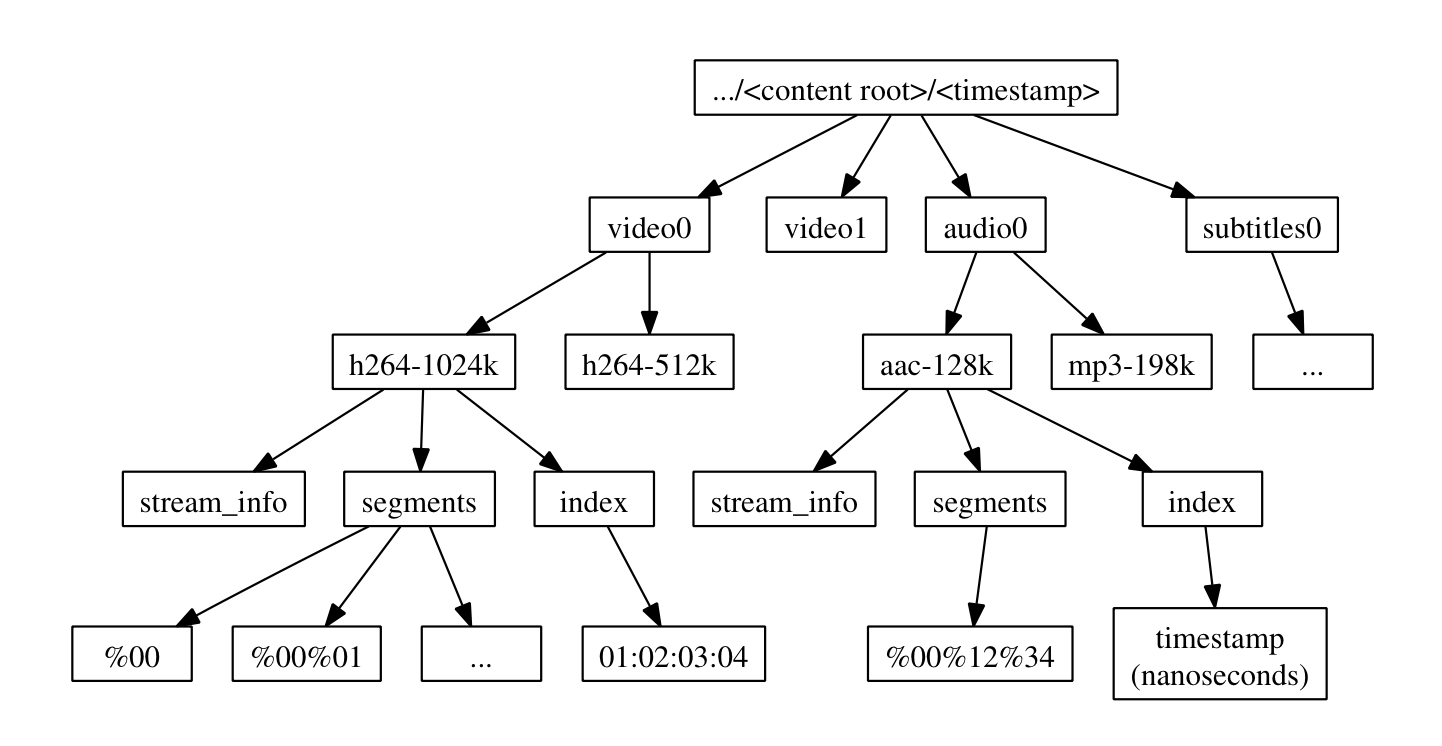
\includegraphics[scale=0.3]{ndnvideo_naming}
  \vspace{-0.3cm}
  \caption{Prior NDNVideo Naming Space}
  \label{fig:ndnvideo_naming}
  \vspace{-0.2cm}
\end{figure}

NDNVideo provides live and pre-recorded video streaming over NDN using Gstreamer library for media processing and Repo for permanent storage~\cite{ndnvideo}. Since the new NFD does not support the previous packet format, this implementation of video streaming is now obsolete.

The major difference between NDNlive~/~NDNtube and NDNVideo is the organization of the video and audio content. In the NDNVideo, video or audio streams are chopped into fixed-size segments, which requires a special mapping between real playback time and segment numbers to keep video and audio synced, and support ``seek'' functionality (Figure~\ref{fig:ndnvideo_naming}). Fixed-size segmentation breaks the boundaries of frames (e.g. Application Data Units), which causes the inter-dependency between different frames leading to the problems inherent to TCP/IP such as Head-Of-Line (HOL) blocking.

In NDNlive and NDNtube, video and audio streams are chopped into frames. One frame may contain several segments. Since segmentation is provided by Consumer / Producer API, it is transparent for the application, which has to focus only at frame level. Since every frame has a unique name and is independent from any other frames, any missing frames do not affect other frames, which is highly beneficial for video streaming applications, especially for live streaming applications. For example, in NDNLive, if the previous frame can't be retrieved on time, the consumer can just skips it and continues with the next frame to keep the video streaming. 

Table~\ref{table:comparison} illustrates other significant differences such as library dependencies and versions, and programming languages.

\begin{table}[ht]	
	\begin{tabular}{|c|c|c|}
	\hline
	             & NDNLive \& NDNTube                                                              & NDNVideo                                                     \\ \hline 
	Dependencies & \begin{tabular}[c]{@{}c@{}}ndn-cxx / NFD\\ Consumer / Producer API\end{tabular} & \begin{tabular}[c]{@{}c@{}}CCNx / CCNR \\ pyccn\end{tabular} \\ \hline
	Gstreamer    & 1.x                                                                             & 0.1                                                          \\ \hline
	Framing      & video \& audio frames                                                           & fixed segments                                               \\ \hline
	Language     & c++                                                                             & python                                                       \\ \hline
	\end{tabular}
	\caption{Comparison with NDNVideo}
	\label{table:comparison}
\end{table}
